\chapter{Language Design and Syntax Specification}
\label{ch:lang_design}

\section{Design Philosophy and Developer Ergonomics}
\label{sec:design_philosophy}

The primary objective of \ToposLang{} ($\tau$-\textbf{Lang}) is to provide a programming environment where multi-dimensional topology and continuous geometry are first-class language constructs, rather than simulated through numerical approximations or ad-hoc pointer graphs. The design of \ToposLang{} is governed by four core principles:

\begin{enumerate}[leftmargin=1.2cm]
    \item \textbf{Coordinate-Free Geometric Primitives:}  
    In classical languages, working with spatial geometry requires developers to explicitly manage Cartesian coordinate systems ($x, y, z$), matrix transformation conventions (row-major versus column-major), and orientation representations (Euler angles vs.\ quaternions). In \ToposLang{}, geometric entities (points, lines, planes, spheres) and transformations (rotations, translations, scaling) are represented natively as graded Clifford multivectors. Developers manipulate geometry coordinate-free via invariant algebraic operations: the geometric product, the inner contraction, the outer wedge product, and versor/motor sandwiching.

    \item \textbf{Axiomatic Structural Safety via Boundary Nilpotency:}  
    Memory safety in \ToposLang{} is enforced at the topological level. The compiler statically verifies that every cell, chain, and cellular rewrite preserves the fundamental topological axiom of boundary nilpotency:
    \begin{equation}
        \partial^2 = 0
    \end{equation}
    An attempt to construct a malformed geometric shape, attach an inconsistent face, or define a rewrite between non-parallel boundary chains triggers a static compiler error before intermediate code generation begins. Data corruption is syntactically unrepresentable.

    \item \textbf{Homotopy as First-Class State Transformation:}  
    Computation does not proceed through destructive in-place register overwriting. State transitions are declared as cellular homotopies that attach higher-dimensional cells to bridge computational input and output states. This preserves execution history as geometric depth, facilitating deterministic execution, reversible computing, and total spatial traceability.

    \item \textbf{Invariant-Driven Control Flow:}  
    Instead of heuristic loop termination ($\|x_{k+1} - x_k\| < \epsilon$), \ToposLang{} provides native control structures governed by topological invariants: the Betti numbers $\beta_k$ and the Euler characteristic $\chi$. Loops execute until structural obstructions vanish ($\texttt{until betti(K, dim=k) == 0}$), providing compile-time and runtime guarantees of deadlock freedom and consensus resolution.
\end{enumerate}

\subsection{The Developer Mental Model: From Register Overwriting to Spatial Tesselation}
\label{subsec:mental_model}

To program effectively in \ToposLang{}, software engineers shift from a temporal register-mutation mental model to a spatial-topological mental model:

\begin{itemize}[leftmargin=1.2cm]
    \item \textbf{The Imperative Mental Model (Classical C / Assembly):}  
    \textit{``I have a memory address $\texttt{0x7ffee4}$. I read its 64-bit value into register $\texttt{RAX}$, increment it, and overwrite $\texttt{0x7ffee4}$. If another thread attempts to read this address simultaneously, I must acquire a spinlock to block that thread.''}
    
    \item \textbf{The Functional Mental Model (Haskell / OCaml):}  
    \textit{``I have an immutable data structure $S$. I apply a pure function $f(S)$ to yield a newly allocated data structure $S'$. I sequence effects through a monadic bind ($\gg=$) which forces step $B$ to await the completion of step $A$.''}

    \item \textbf{The Topological Mental Model (\ToposLang{}):}  
    \textit{``I have an active topological cell complex $\mathcal{K}$. Vertices ($\texttt{cell0}$) represent system states or agents. Directed edges ($\texttt{cell1}$) represent transactions or processes. When process $A \to B$ and process $B \to C$ occur, an open loop is formed with alternative path $A \to C$. I apply a homotopy rewrite $\texttt{(e1 + e2) => e3}$, which attaches a 2-dimensional cell ($\texttt{cell2}$) to seal the triangle. The attached surface proves that the paths are equivalent and completes the transaction. If two transactions act on disconnected spatial sub-complexes, they run concurrently with zero locks. I terminate my coordination loop when $\texttt{betti(1) == 0}$, guaranteeing that all communication deadlocks have been closed.''}
\end{itemize}

This conceptual reorientation makes distributed coordination, concurrent synchronization, and geometric transformations direct physical consequences of data representation.

---

\section{Grammar and Concrete Syntax Specification}
\label{sec:grammar_syntax}

We formalize the syntax of \ToposLang{} using Extended Backus-Naur Form (EBNF). The language grammar is structured into four layers: top-level modules, cellular declarations, algebraic rewrite rules, and invariant control processes.

\subsection{EBNF Grammar}
\begin{lstlisting}[language={}]
Program            ::= ( Declaration | ProcessDef )* EOF

Declaration        ::= HITDef
                     | CellDef
                     | ChainDef
                     | RewriteDef
                     | MotorDef

HITDef             ::= "hit" Identifier "{" HITMember* "}"
HITMember          ::= "point" Identifier ";"
                     | "path" Identifier ":" PathExpr "=" PathExpr ";"
                     | "surface" Identifier ":" PathExpr "=" PathExpr ";"

CellDef            ::= "cell" IntegerLiteral Identifier ( ":" CellBoundary )? ";"
CellBoundary       ::= ChainExpr "->" ChainExpr
                     | "{" FaceList "}"
FaceList           ::= FaceEntry ( "," FaceEntry )*
FaceEntry          ::= Identifier ":" IntegerLiteral

ChainDef           ::= "chain" IntegerLiteral Identifier "=" ChainExpr ";"
ChainExpr          ::= Term ( ( "+" | "-" ) Term )*
Term               ::= ( RationalLiteral | MultivectorLiteral )? ( "*" )? Identifier

RewriteDef         ::= "rewrite" Identifier ":" "(" ChainExpr ")" "=>" "(" ChainExpr ")" ";"

ProcessDef         ::= "process" Identifier "(" ParamList ")" "{" ProcessStmt* "}"
ParamList          ::= Param ( "," Param )*
Param              ::= Identifier ":" TypeName
TypeName           ::= "CellComplex" | "Chain" | "Multivector" | "Motor"

ProcessStmt        ::= ApplyStmt
                     | InvariantLoop
                     | LetStmt
                     | MotorTransformStmt

ApplyStmt          ::= "apply" Identifier "on" Identifier ";"
InvariantLoop      ::= "until" InvariantExpr "{" ProcessStmt* "}"
InvariantExpr      ::= "betti" "(" Identifier "," "dim" "=" IntegerLiteral ")" "==" IntegerLiteral
                     | "euler" "(" Identifier ")" "==" IntegerLiteral

MotorDef           ::= "motor" Identifier ":" AlgebraSig "=" MotorExpr ";"
AlgebraSig         ::= "PGA" "(" IntegerLiteral "," IntegerLiteral "," IntegerLiteral ")"
                     | "CGA" "(" IntegerLiteral "," IntegerLiteral "," IntegerLiteral ")"
                     | "Clifford" "(" IntegerLiteral "," IntegerLiteral "," IntegerLiteral ")"

MotorTransformStmt ::= "sandwich" Identifier "with" Identifier ";"
\end{lstlisting}

---

\section{Compiler Pipeline Architecture}
\label{sec:compiler_pipeline}

The \ToposLang{} compilation infrastructure lowers high-level topological specifications into hardware-executable instructions through a five-stage progressive lowering pipeline built on the Multi-Level Intermediate Representation (MLIR) framework \cite{lattner2021mlir}.

\begin{figure}[h]
\centering
\small
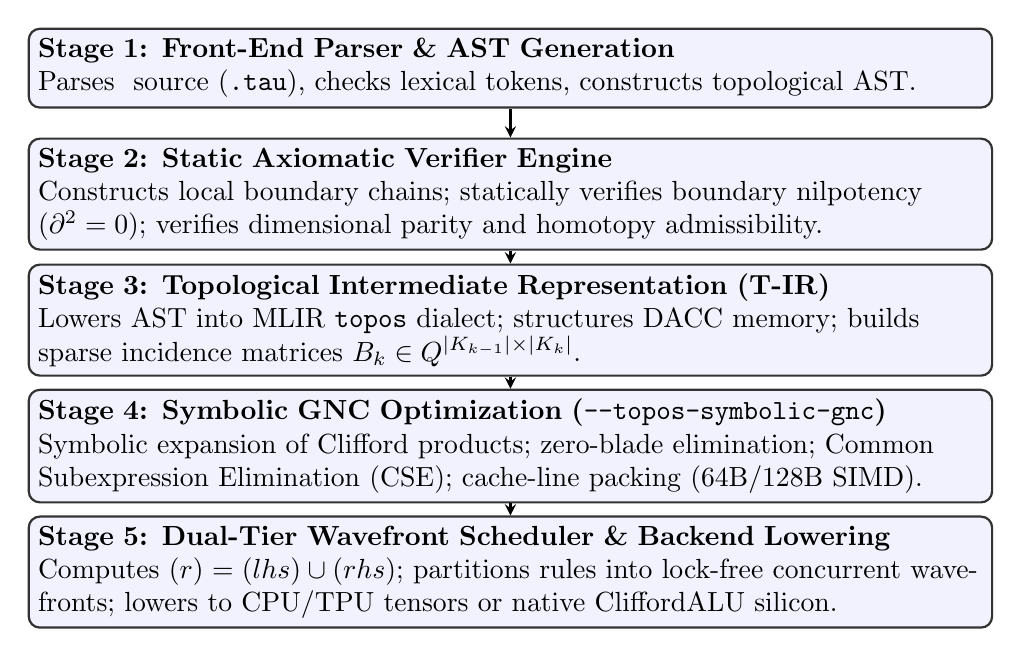
\begin{tikzpicture}[node distance=1.6cm, auto,
    block/.style={rectangle, draw=black!80, fill=blue!5, thick, text width=12cm, minimum height=1cm, rounded corners},
    arrow/.style={thick, ->, >=stealth}]

    \node [block] (frontend) {\textbf{Stage 1: Front-End Parser \& AST Generation}\\
    Parses \ToposLang{} source (\texttt{.tau}), checks lexical tokens, constructs topological AST.};
    
    \node [block, below of=frontend] (verifier) {\textbf{Stage 2: Static Axiomatic Verifier Engine}\\
    Constructs local boundary chains; statically verifies boundary nilpotency ($\partial^2 = 0$); verifies dimensional parity and homotopy admissibility.};
    
    \node [block, below of=verifier] (tir) {\textbf{Stage 3: Topological Intermediate Representation (T-IR)}\\
    Lowers AST into MLIR \texttt{topos} dialect; structures DACC memory; builds sparse incidence matrices $B_k \in \mathbb{Q}^{|K_{k-1}| \times |K_k|}$.};
    
    \node [block, below of=tir] (opt) {\textbf{Stage 4: Symbolic GNC Optimization (\texttt{--topos-symbolic-gnc})}\\
    Symbolic expansion of Clifford products; zero-blade elimination; Common Subexpression Elimination (CSE); cache-line packing (64B/128B SIMD).};
    
    \node [block, below of=opt] (wavefront) {\textbf{Stage 5: Dual-Tier Wavefront Scheduler \& Backend Lowering}\\
    Computes $\supp(r) = \cl(\text{lhs}) \cup \cl(\text{rhs})$; partitions rules into lock-free concurrent wavefronts; lowers to CPU/TPU tensors or native CliffordALU silicon.};

    \draw [arrow] (frontend) -- (verifier);
    \draw [arrow] (verifier) -- (tir);
    \draw [arrow] (tir) -- (opt);
    \draw [arrow] (opt) -- (wavefront);
\end{tikzpicture}
\caption{The Five-Stage \ToposLang{} / GNC Compiler Lowering Pipeline.}
\label{fig:compiler_pipeline}
\end{figure}

\subsection{Detailed Architectural Stages}

\subsubsection{Stage 1: Front-End Ingestion and AST Generation}
The compiler front-end ingests \ToposLang{} source files ($\texttt{.tau}$). The lexer tokenizes topological keywords (\texttt{hit}, \texttt{cell0}, \texttt{cell1}, \texttt{rewrite}, \texttt{until}, \texttt{betti}, \texttt{motor}). The recursive-descent parser constructs an Abstract Syntax Tree (AST) where nodes correspond to graded cells, chain linear combinations, cellular rewrite homotopies, and invariant loops.

\subsubsection{Stage 2: Static Axiomatic Verification Engine}
Before any code generation occurs, the axiomatic engine checks every declaration:
\begin{enumerate}
    \item \textbf{Dimensional Consistency:} In any rewrite rule $r : \text{lhs} \Rightarrow \text{rhs}$, the compiler asserts:
    \begin{equation}
        \dim(\text{lhs}) = \dim(\text{rhs}) = k
    \end{equation}
    \item \textbf{Parallel Boundary Condition:} The compiler computes the boundary chain of both sides and verifies:
    \begin{equation}
        \partial_k(\text{rhs}) - \partial_k(\text{lhs}) = 0
    \end{equation}
    \item \textbf{Boundary Nilpotency Verification:} For the newly attached $(k+1)$-cell $\alpha_r$ with boundary $\partial \alpha_r = \text{rhs} - \text{lhs}$, the verifier evaluates:
    \begin{equation}
        \partial_k(\partial_{k+1}(\alpha_r)) = 0
    \end{equation}
    If this condition fails, the compiler halts with an axiomatic error diagnostic, detailing the non-closed residual chain.
\end{enumerate}

\subsubsection{Stage 3: Topological Intermediate Representation (T-IR)}
The validated AST is lowered into the \texttt{topos} MLIR dialect. In this stage:
\begin{itemize}
    \item Cell identifiers are mapped to graded 64-bit integer registers;
    \item Boundary relationships are materialized as exact sparse integer incidence matrices $B_k \in \mathbb{Q}^{|K_{k-1}| \times |K_k|}$;
    \item Cell complexes are encapsulated in state containers maintaining homology caches.
\end{itemize}

\subsubsection{Stage 4: Symbolic GNC Optimization Pass (\texttt{--topos-symbolic-gnc})}
When multivector operations are present, naively performing dense matrix multiplication of $2^n$-dimensional multivectors would incur $O(2^{2n})$ operations. The \texttt{--topos-symbolic-gnc} pass:
\begin{itemize}
    \item Evaluates basis blade interactions symbolically at compile time;
    \item Propagates structural zeroes, pruning absent blades (e.g., in 3D PGA, points and planes require only 4 non-zero coefficients rather than 16);
    \item Emits vectorized, flat scalar arithmetic in MLIR \texttt{llvm} and \texttt{vector} dialects, aligned to 64-byte (x86 AVX-512) or 128-byte (ARM SME) cache lines.
\end{itemize}

\subsubsection{Stage 5: Dual-Tier Spatial Wavefront Scheduling}
The runtime scheduler queries the spatial support closures $\supp(r) = \cl(\text{lhs}) \cup \cl(\text{rhs})$ for all pending rewrite rules. Spatially disjoint rules are grouped into independent concurrent execution wavefronts. If discrete supports overlap, the scheduler evaluates the continuous multivector wedge product $S_1 \wedge S_2$. Disjoint operations are dispatched across CPU threads or TPU execution cores with \textbf{zero mutex locks and zero thread barriers}.

---

\section{Canonical Example Programs and Idioms}
\label{sec:canonical_programs}

To illustrate the concrete syntax, abstractions, and developer ergonomics of \ToposLang{}, we present four complete, canonical programs.

\subsection{Example 1: Higher Inductive Types ($S^1$ and Torus $T^2$)}
This program demonstrates the definition of topological spaces as Higher Inductive Types, establishing topological boundary loops and 2-dimensional surface contracts.

\begin{lstlisting}[caption={Higher Inductive Types for Circle $S^1$ and Torus $T^2$ in \ToposLang{}.}]
// Module: TopologyPrimitives.tau
// Demonstrating Higher Inductive Types (HITs)

// Definition of the topological circle S1
hit S1 {
    point base;
    path loop : base = base;
}

// Definition of the 2-dimensional Torus T2
hit Torus {
    point b;
    path p : b = b;
    path q : b = b;
    surface face : (p * q) = (q * p);
}

// The torus surface constructor proves the commutativity of fundamental loops:
// p * q * p^-1 * q^-1 = 1
\end{lstlisting}

\subsection{Example 2: Invariant-Driven Vortex Loop Contraction}
This program models a 2-dimensional triangular simplicial complex containing an open 1-dimensional cycle (a topological hole or vortex). The program applies a cellular homotopy rewrite to fill the void, terminating when the first Betti number $\beta_1$ vanishes.

\begin{lstlisting}[caption={Invariant-Driven Vortex Contraction on a 2-Simplex.}]
// Module: VortexContraction.tau
// Topological cell definitions for a 2-simplex boundary
cell0 A;
cell0 B;
cell0 C;

// Directed 1-cells (edges forming an open cycle)
cell1 e1 : A -> B;
cell1 e2 : B -> C;
cell1 e3 : A -> C;

// Initially, the complex has:
// Vertices |K0| = 3, Edges |K1| = 3, Faces |K2| = 0
// beta_0 = 1 (one connected component)
// beta_1 = 1 (one open 1-cycle: e1 + e2 - e3)

process contract_vortices(complex: CellComplex) {
    // Define the cellular homotopy rewrite:
    // Replaces path (e1 + e2) with direct edge e3 by attaching 2-cell alpha
    rewrite loop_contraction : (e1 + e2) => e3;

    // Invariant-driven control loop:
    // Terminates deterministically when the 1st Betti number reaches 0
    until betti(complex, dim=1) == 0 {
        apply loop_contraction on complex;
    }
}
\end{lstlisting}

\subsection{Example 3: Distributed Multi-Agent Spatial Coordination Mesh}
This program demonstrates lock-free concurrency across two distributed compute clusters (Cluster Alpha and Cluster Beta). Because the clusters operate on topologically disjoint sub-complexes, the \ToposLang{} compiler and runtime schedule their rewrite rules in a single concurrent wavefront with zero locks.

\begin{lstlisting}[caption={Multi-Agent Spatial Coordination Mesh with Disjoint Execution Wavefronts.}]
// Module: MultiAgentMesh.tau
// Domain Alpha: Cluster A (Compute Pipeline)
cell0 TaskA_Init;
cell0 TaskA_Running;
cell0 TaskA_Done;

cell1 dispatch_A  : TaskA_Init    -> TaskA_Running;
cell1 execute_A   : TaskA_Running -> TaskA_Done;
cell1 reconcile_A : TaskA_Init    -> TaskA_Done;

// Domain Beta: Cluster B (Database Sync Pipeline)
cell0 TaskB_Init;
cell0 TaskB_Running;
cell0 TaskB_Done;

cell1 dispatch_B  : TaskB_Init    -> TaskB_Running;
cell1 execute_B   : TaskB_Running -> TaskB_Done;
cell1 reconcile_B : TaskB_Init    -> TaskB_Done;

// Multi-Agent Invariant-Driven Process
process synchronize_mesh(complex: CellComplex) {
    rewrite resolve_alpha : (dispatch_A + execute_A) => reconcile_A;
    rewrite resolve_beta  : (dispatch_B + execute_B) => reconcile_B;

    // Both rules have disjoint spatial support:
    // supp(resolve_alpha) \cap supp(resolve_beta) == \emptyset
    // The runtime scheduler automatically executes them in parallel without locks.

    until betti(complex, dim=1) == 0 {
        apply resolve_alpha on complex;
        apply resolve_beta on complex;
    }
}
\end{lstlisting}

\subsection{Example 4: Continuous Robotic Kinematics with 3D PGA Motors}
This program demonstrates Geometric Native Coding using 3D Projective Geometric Algebra ($\mathbb{R}^{3,0,1}$). A robotic manipulator arm is defined using multivector motors. Transformations and obstacle collision tests are evaluated using coordinate-free versor sandwiches and closed-form outer wedge intersections.

\begin{lstlisting}[caption={Continuous Robotic Kinematics with PGA Versors and Collision Checking.}]
// Module: RobotKinematics.tau
// 3D Projective Geometric Algebra (PGA R^{3,0,1})

// Define kinematic joints and link planes
motor Joint1_Rot : PGA(3,0,1) = rotor(axis=e12, angle=0.785398); // 45 deg
motor Link1_Trans: PGA(3,0,1) = translator(dir=e03, dist=2.5);

// Combined rigid body motor: M = Trans * Rot
motor ArmMotor : PGA(3,0,1) = Link1_Trans * Joint1_Rot;

// Define end-effector geometric line and obstacle plane
blade EndEffectorLine : PGA(3,0,1) = line(p1=origin, p2=target);
blade ObstaclePlane   : PGA(3,0,1) = plane(nx=1, ny=0, nz=0, d=5.0);

process execute_kinematic_step(complex: CellComplex) {
    // Coordinate-free motor sandwich transformation: L' = M * L * M^-1
    sandwich EndEffectorLine with ArmMotor;

    // Closed-form collision detection via outer wedge product:
    // Point P = Line ^ Plane. If P == 0, line and plane are parallel.
    blade IntersectionPoint = EndEffectorLine ^ ObstaclePlane;

    if norm(IntersectionPoint) > 0.0001 {
        // Physical collision detected in closed algebraic form
        trigger_obstacle_avoidance(complex);
    }
}
\end{lstlisting}

---

\section{Diagnostic Feedback and Compile-Time Verification}
\label{sec:diagnostics}

When a developer violates topological consistency, the \ToposLang{} compiler generates precise, actionable diagnostic errors. Consider an erroneous rewrite rule that attempts to attach an invalid, non-closed boundary face:

\begin{lstlisting}[caption={Erroneous \ToposLang{} Program with Boundary Nilpotency Violation.}]
cell0 V0;
cell0 V1;
cell0 V2;

cell1 e0 : V0 -> V1;
cell1 e1 : V1 -> V2;
cell1 e2 : V0 -> V2;

// Malformed rule: LHS boundary != RHS boundary
// LHS: d(e0 + e1) = (V1 - V0) + (V2 - V1) = V2 - V0
// RHS: d(2*e2)    = 2*(V2 - V0) = 2*V2 - 2*V0
rewrite bad_rule : (e0 + e1) => (2 * e2);
\end{lstlisting}

Upon compilation, the \ToposLang{} static verifier rejects the code with the following diagnostic:

\begin{lstlisting}[language={}, caption={Diagnostic Error Emitted by the \ToposLang{} Compiler.}]
error[E0101]: Topological Boundary Nilpotency Violation (d^2 != 0)
  --> test_err.tau:11:1
   |
11 | rewrite bad_rule : (e0 + e1) => (2 * e2);
   | ^^^^^^^^^^^^^^^^^^^^^^^^^^^^^^^^^^^^^^^^
   |
   = note: The rewrite rule creates a non-closed geometric boundary attachment.
   = detail: Input LHS boundary:  +1*V2 - 1*V0
             Target RHS boundary: +2*V2 - 2*V0
             Residual Boundary:   +1*V2 - 1*V0 != 0
   = axiom: Fundamental Axiom 1.1 dictates that d(RHS - LHS) == 0.
   = help: Ensure that LHS and RHS chains share identical oriented boundary faces.
\end{lstlisting}

This compile-time diagnostic guarantees that invalid topological operations are intercepted before program lowering, ensuring absolute structural safety.
